%
\section{The Fundamental Data Structures within MultiRegions}

As mentioned earlier, in almost all object-oriented languages (which includes $C++$), there exists the concepts of {\em class attributes} and {\em object attributes}.   For a summary of attributes and access patterns, please review Section \ref{sec:stdregions-datastructures}.
Within the MultiRegions directory of the library, there exists a class inheritance hierarchy designed to try to encourage re-use of core
algorithms (while simultaneously trying to minimize duplication of code).  We present this class hierarchy in Figure \ref{multiregions:multiregionstree}.


\begin{figure}[htb]
\centering
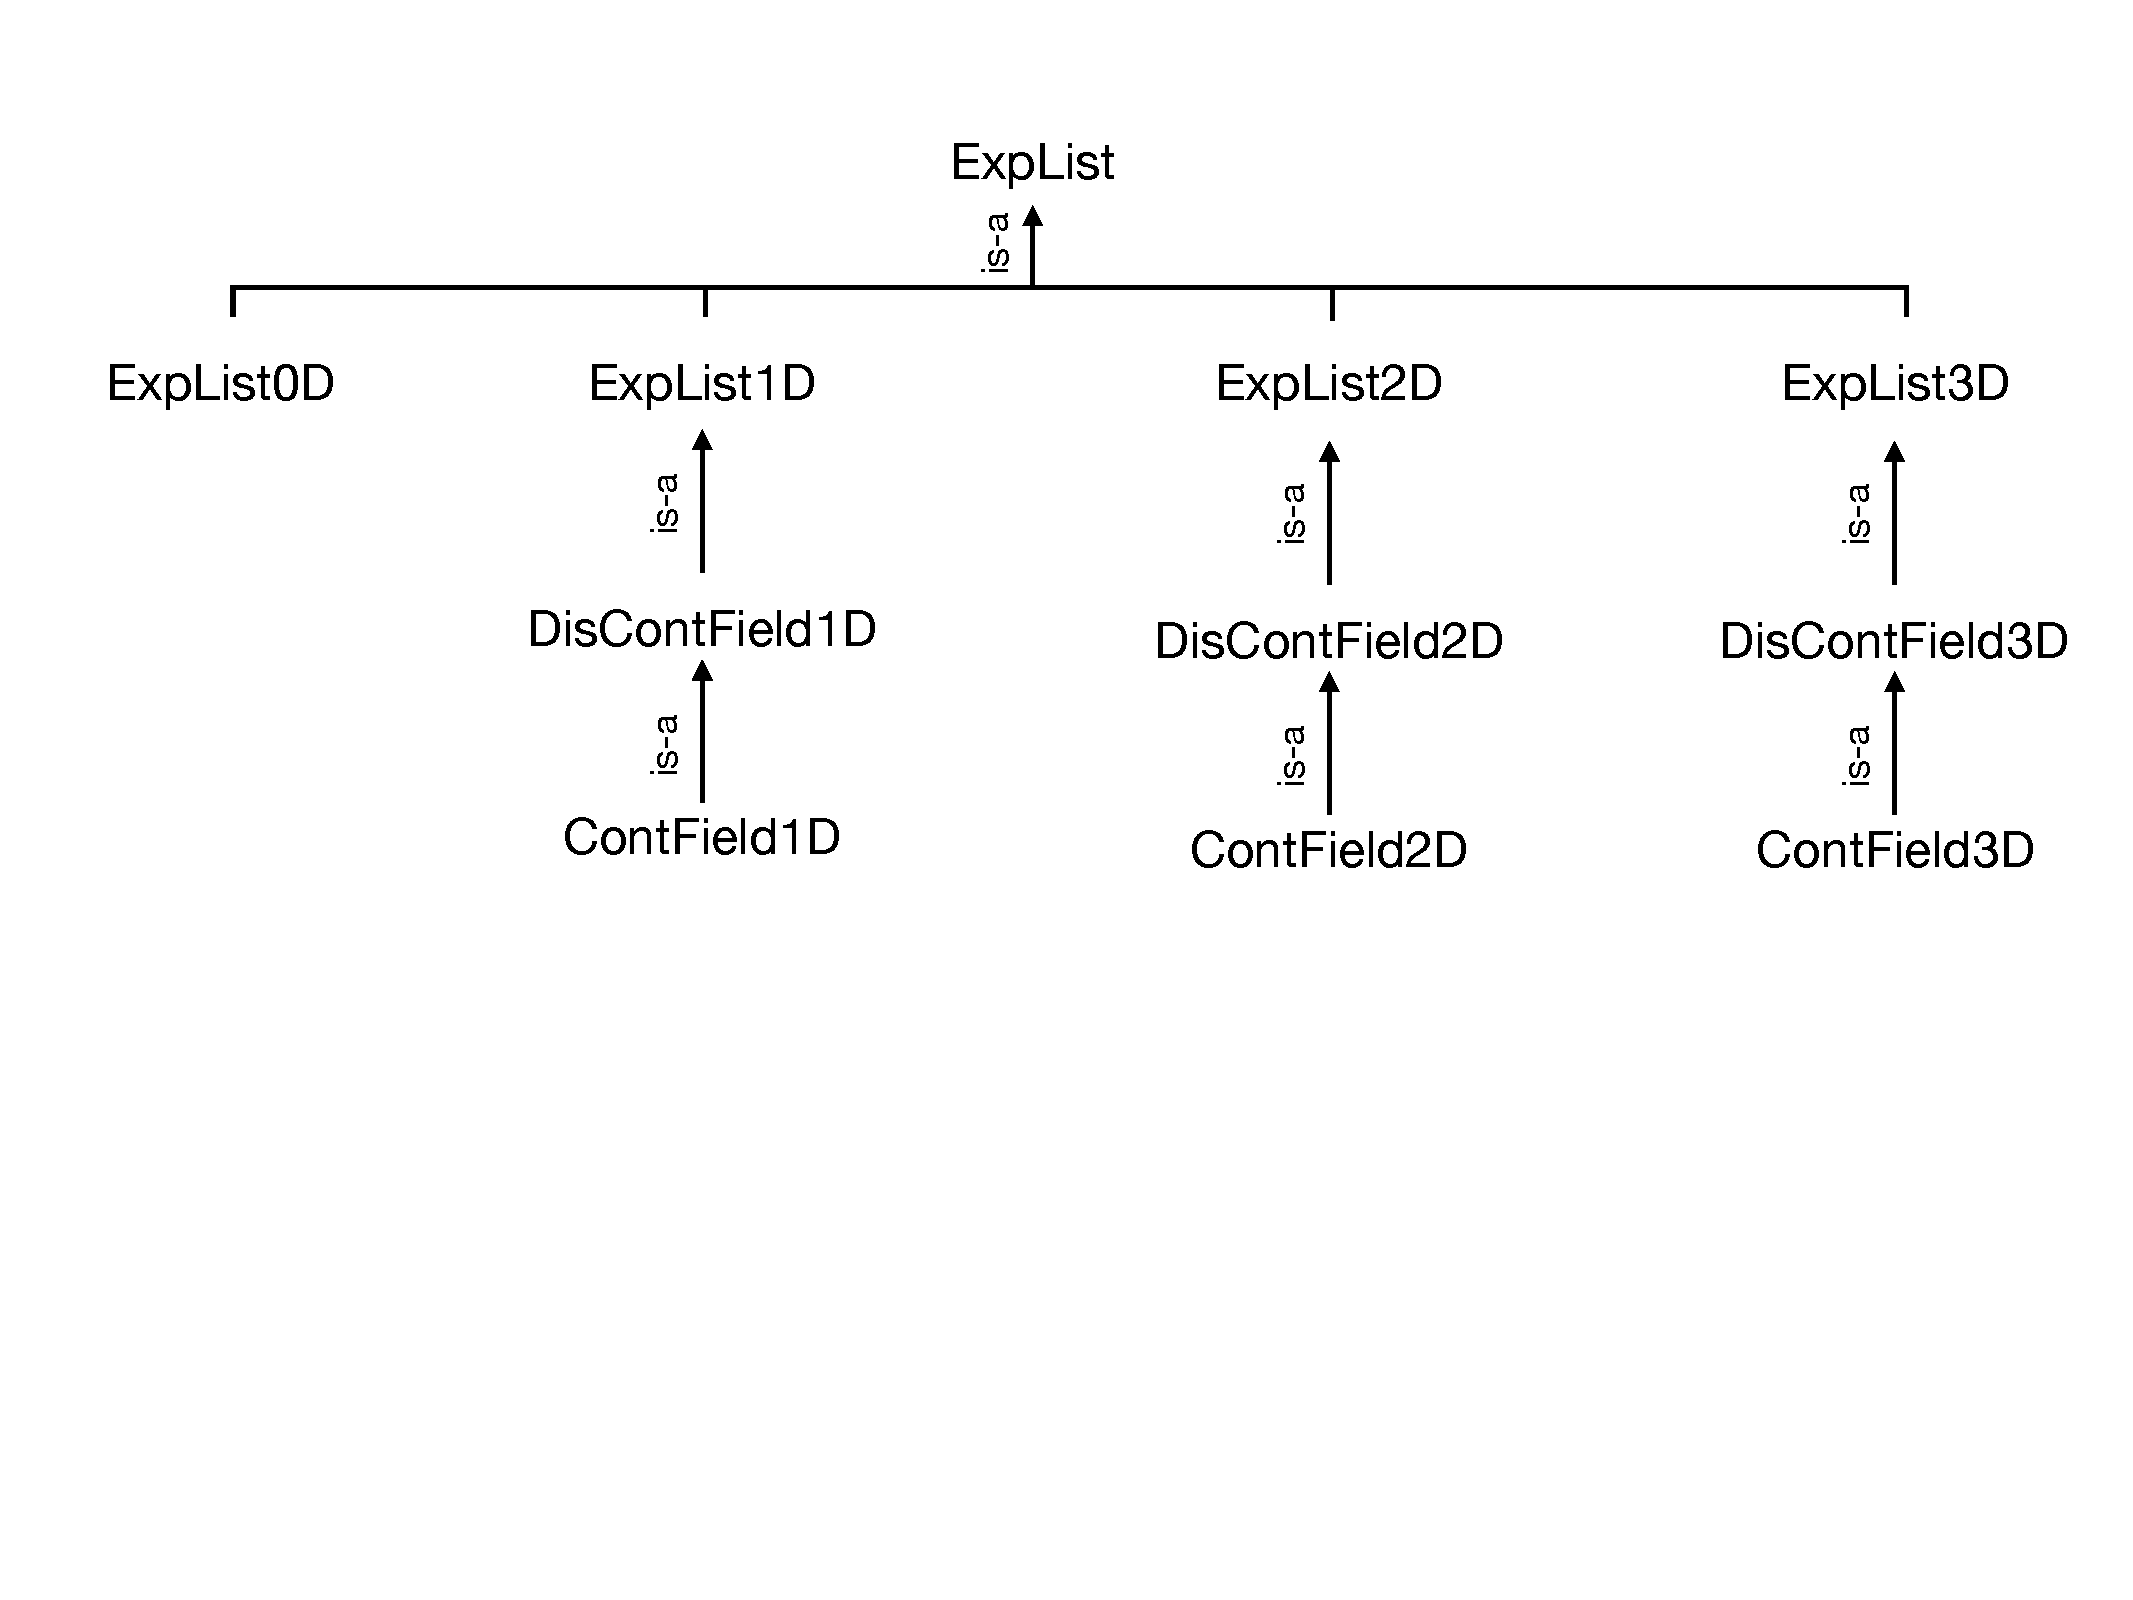
\includegraphics[width=6in]{img/multiregiontree.pdf}
\caption{Class hierarchy derived from ExpList, the base class of the MultiRegions Directory.}
\label{multiregions:multiregionstree}
\end{figure}

At its core, the items contained within MultiRegions are meant to represent sets of LocalRegions.  In the most abstract sense, an 
ExpList is merely a set of LocalRegion objects that may or may not have any relevance to each other.   We then, as we do in 
other parts of the library, specialize on the dimension of the objects these sets will contain.  At the subsequent levels of the
hierarchy, we now involve information about we want to treat a collection of elements when evaluating them as a {\em field}.  
We consider a {\em field} to be the representation of a function over a (sub--)domain.  A domain consists of a collection of elements
that are {\em connected} (that is, they form a contiguous region in space).   We think of the region of space as being tiled by elements
over which expansions are build.  If we consider a MultiRegion field to be a collection of these expansions with no constraints on their
continuity, we arrive at the DisContField family of class definitions (which vary by dimension).  For the currently available solvers within
{\nek}, this level of field is used for the solution of PDEs via the discontinuous Galerkin (dG) and Flux-Reconstruction (FR) methods.
If we consider a function as a collection of expansion in which we require continuity (in {\nek}, only $C^0$ continuity), then we employ
a further derived class called ContField (which again varies by dimension).  For the currently available solvers
within {\nek}, this level of field is used for the solution of PDEs via the continuous Galerkin (cG) method.
Since many of the operations at the continuous field level do not rely upon the continuity of the field, we have structured the
continuous MultiRegion object as with an {\em is-a} relationship with the DisContFields.

The various private, protected and public data members contained within MultiRegions are provided in the subsequent sections.


%%%%%%%%%%%%%%%%%%%%%%%%%%%%%%%%%%%%%%%%
\subsection{Variables at the Level of ExpList}

\paragraph{Private:}

\paragraph{Protected:}

\paragraph{Public:}


%%%%%%%%%%%%%%%%%%%%%%%%%%%%%%%%%%%%%%%%
\subsection{Variables at the Level of ExpList\$D for various Dimensions}

\paragraph{Private:}

\paragraph{Protected:}

\paragraph{Public:}


%%%%%%%%%%%%%%%%%%%%%%%%%%%%%%%%%%%%%%%%
\subsection{Variables at the Level of Discontinuous Field Expansions}

\paragraph{Private:}

\paragraph{Protected:}

\paragraph{Public:}


%%%%%%%%%%%%%%%%%%%%%%%%%%%%%%%%%%%%%%%%
\subsection{Variables at the Level of Continuous Field Expansions}

\paragraph{Private:}

\paragraph{Protected:}



